\section{Methodology}

This section outlines the techniques, tools, and procedures used to build a vision-aided shopping list system. The entire system was developed using AWS tools, which facilitate integration, scalability, and support, as all services come from the same provider.

The tools utilized are: 
\begin{itemize} 
	\item Amazon DynamoDB, for the creation and management of the database. 		\item Amazon Rekognition, for product recognition through input images. 		\item Alexa Skills Kit (ASK), for developing the Skill that will allow users to interact with the system via Alexa. 
	\item AWS Lambda, to integrate the previously mentioned tools. 
\end{itemize}

The methodology is divided into three main parts: 
\begin{itemize} 
	\item Database Creation and Structuring
	\item Real-time Product Recognition 
	\item Integration with the Alexa Virtual Assistant 
\end{itemize}

\subsection{Database Structure}

The database's function in this project is to store the products available in the store, which need to be updated periodically. The goal is to allow users to check what products are in stock and their quantities in near real-time.

The table, named \texttt{ProductsList}, was structured as follows: \begin{itemize} 
	\item \textbf{Primary Key}: The primary key is the 
	\texttt{ProductName} attribute, which is a string (S) type. This uniquely identifies each item in the table. 
	\item \textbf{Attributes}: The table contains the following attributes: \begin{itemize} 
		\item \texttt{ProductName} (string) – The name of the product, serving as the primary key. 
		\item \texttt{Brand} (string) – The brand of the product. 
		\item \texttt{Quantity} (number) – The available quantity of the product. 
		\item \texttt{Category} (string) – The category to which the product belongs (e.g., Dairy, Bakery, Snacks). 
	\end{itemize} 
\end{itemize}

Access to the table is done via AWS Lambda functions, both for reading and writing data. These functions use the boto3 library, a Python SDK created to manage AWS resources.

\subsection{Product Recognition with Amazon Rekognition}

For product recognition using Amazon Rekognition, it is necessary to create a dataset using an S3 bucket to train the model that will identify the products. Once the dataset is created, we configure SageMaker, where labels will be generated for each product. These labels will be used to identify the products in each image within the dataset.

Next, the model will be trained using Amazon Rekognition Custom Labels. The labeled images from SageMaker Ground Truth will be imported through the manifest file location that was provided when the S3 bucket was created.

Once the model training is complete, the model will be deployed using Lambda. To achieve this, the commands listed in Appendix \ref{appendix:recognition_lambda} must be executed using the AWS CLI.



\subsection{Alexa Skill Integration}

To enable users to check the store's stock via the Alexa virtual assistant, a custom Alexa Skill was developed. Skills are essentially extensions or applications for Alexa that serve specific purposes. In this case, the Skill queries the previously created database to provide personalized responses based on voice commands with specific keywords.

The Skill was created using the command-line interface (CLI) provided by ASK. Initially, the Skill named \texttt{ProductListSkill} was created using the "Hello World" Lambda function template. Then, three key files were modified:

\begin{itemize} 
	\item \texttt{interactionModels/custom/en-US.json}: This file contains the definition of intents and sample interactions (Appendix \ref{appendix:interaction}). 
	\item \texttt{skill-package/skill.json}: This file holds the basic configuration of the Skill (Appendix \ref{appendix:skill_config}).
	\item \texttt{lambda/hello-world.py}: The Lambda function written in Python to access the previously created database (Appendix \ref{appendix:lambda}).
\end{itemize}

In addition, the Lambda function must be granted permission to access DynamoDB. The created Skill can inform users about the stock levels of specific products and list all available products.

The initial tests were conducted using the ASK CLI. It’s possible to start a dialogue via the command line using the 'ask dialog' command. To use the Skill, users must first invoke it by saying, "open products list," and then use one of the sample commands defined in the \texttt{en-US.json} file, such as “list all products.” An example of the testing process is shown in Figure \ref{ask-cli}.

\begin{figure}[h] 
	\centering 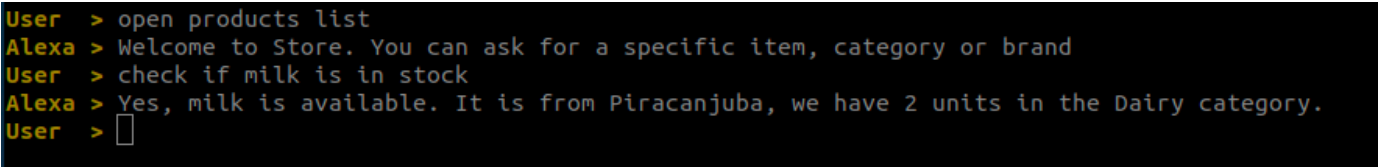
\includegraphics[width=\textwidth]{images/ask-cli} 					\caption{Testing Alexa Skill with ASK-CLI.} 
	\label{ask-cli} 
\end{figure}

